\chapter{Implementation}
\label{chap:implementation}

To feed the batch optimization, data needs to be collected.
In this work we used both data from simulation and from a real blimp.
In this chapter we will first define what a dataset is and then 
describe the methods used to generate these datasets from a real blimp and also from simulation.

\section{Dataset}
\label{sec:dataset}
The \textsc{MATLAB} implementation of the batch optimisation takes a dataset as the input and returns a set of optimal parameters estimated from the given dataset. \\
A dataset is designed to be self contained. 
Each dataset includes information about the structure of the system and a set of input vectors with their corresponding measurement vectors from the sensors. \\
In the current implementation the structure contains the true values
\footnote{True values are only known for the simulation datasets. 
For datasets from the real blimp, the true values are not known and therefore replaced with values based on the CAD files of the blimp}
for the motor positions and their coordinate system transformations, the blimp radius, the blimp mass and the inertial tensor as well as transformation matrices for the sensors. \\
The measurement data is stored in segments.
A segment is a homogeneous sequence of continuously sampled actuator feedback vectors as well as measurement vectors.
Because the real system exhibits transients upon changing inputs a boolean is also stored for each data-point which denotes whether the system has reached steady-state. \\
With this technique it is possible to easily cut away parts of segments which have disturbances in them while still preserving transient information.

\section{Real System}
\label{sec:real_system}
To record data from a real blimp, experiments where conducted on the Skye System. \\
To excite the system with actuator inputs which are suitable for batch optimisation we expanded both QGroundControl and the Skye specific PX4 Firmware with new functionality.

\subsection{Input Patterns}
\label{sub:input_pattern}
We tried a number of different approaches to input patterns. \\
The basic idea behind the patterns is that we can apply each of these patterns independently to each other to the blimp.
This allows us to reposition the blimp in the testing area as soon as it drifts away too much.
In order to be able to apply as long of a sequence as possible the individual patterns need to be designed to not build up too much kinetic energy.\\
Another aspect of the real system is that it takes time until the actuators have reached the desired orientation and thrust.
The resulting transients are very hard to predict mainly because the thrust motor controller has no feedback and exhibits very high variability in its dynamic behaviour. \\
In addition to the unknown thruster dynamics the hull also reacts to load changes with vibrations that are detected by the sensors. \\
By combining these constraints on the inputs, we came up with the following pattern scheme:
\begin{enumerate}
\item Apply input vector to system for a fixed amount of time
\item Stop thrust and turn actuators in the opposite direction
\item Apply same inputs in reverse for the same amount of time
\end{enumerate}
Using this scheme the system does not move too much while still providing good steady-state system response. \\
For the input vectors themselves we considered a few options:\\
\begin{enumerate}
\item generate random desired angular accelerations and use allocation to generate input vectors for the thrusters, which result in only rotational acceleration
\item use fixed thrust and select thruster angle from a uniform random number distribution
\item randomize thrust from a random number sequence with given mean and standard deviation and select thruster angle from a uniform random number distribution
\end{enumerate}
The idea behind 1. is to further reduce the amount the blimp moves by removing the translatory forces all together. 
However this approach does not work.\\
The allocation is designed to solve the $\mathbf{M}^{actuation}$ part of the moments equation~\ref{eq:moments} and produce a mapping $\mathbf{M}^{actuation} \rightarrow \mathbf{F}^k_{m_k}$.(??ref to some skye work??)\\
In \ref{eq:m_actuation} the $\mathbf{M}^{actuation}$ part is repeated for convenience.

\begin{equation}
\label{eq:m_actuation}
\mathbf{M}^{actuation} = \sum_{k=1}^N  \left[  \mathbf{C}_{b,m_k} \left( \mathbf{p}^{m_k,cog}_{m_k} \times \mathbf{F}^k_{m_k} \right)  \right]
\end{equation}

It becomes clear that if we use the allocation to feed $\mathbf{F}^k_{m^k}$, $\mathbf{C}_{b,m^k}$ and $\mathbf{p}^{m^k,cog}_{m^k}$ are completely unobservable.\\
This leaves us with methods 2 and 3.
It turns out that fully random method is better than the other one, because method 2 still only excites a limited sub-space of the input space. This is avoided with the fully random inputs provided by method 3.\\

\subsection{Input Generation}
\label{sub:input_generation}
To avoid having to re-flash the firmware all the time, the inputs are generated inside \textsc{QGroundControl} and transmitted with a special direct actuator control message to the blimp.
The firmware then just forwards the actuator commands to the actuators. \\
This way all of the parameters like standard deviation and time intervals can be set from within the \textsc{QGroundControl} interface.

\begin{figure}[hbtp]
\centering
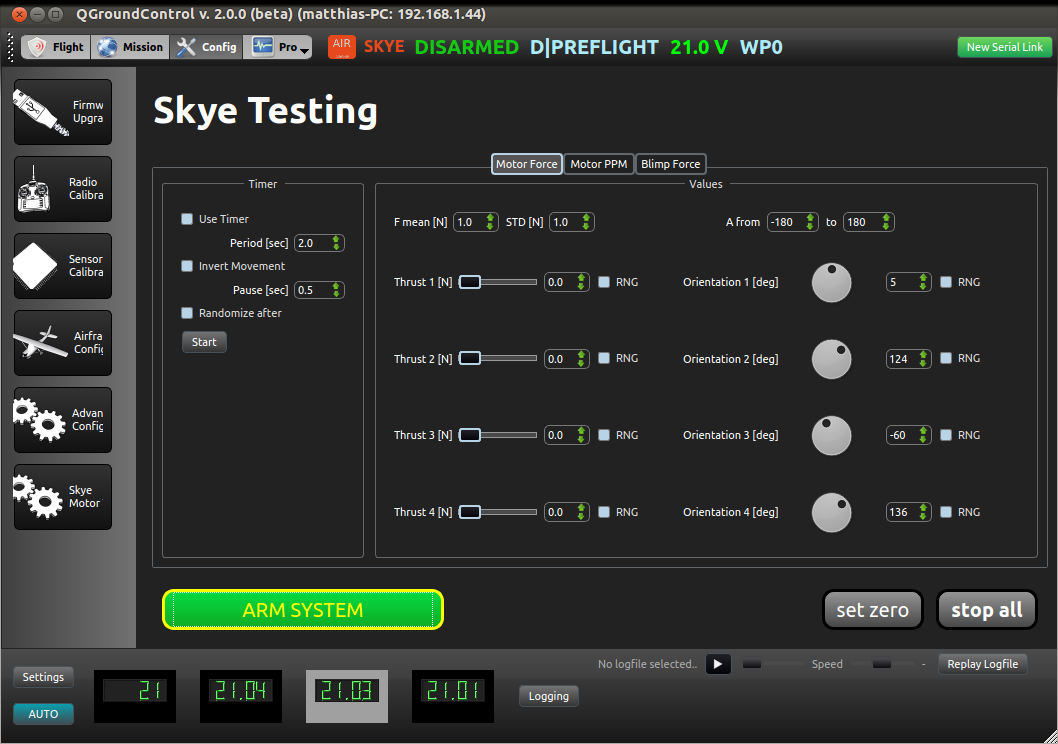
\includegraphics[width=.9\linewidth]{images/qgc/QGroundControl_v_2.png}
\caption{\textsc{QGroundControl} System input generation interface}
\label{fig:qgc_input_gen}
\end{figure}

\subsection{Testing Setup}
\label{sub:testing_setup}
Although the input patterns are designed to avoid large movements as good as possible, the blimp still needs to be catched after a number of such inputs. This leads us to the basic testing setup we used to record data: \\
An operator is located at the ground station and a second operator is near the blimp.
At the ground station there is a button to initiate one such input sequence.
The operator at the blimp catches it as soon as it drifts too close to an obstacle. \\
With this setup it was possible to initiate an input sequence roughly every 6 seconds. 
This is including the time needed to reposition the blimp when it has drifted too much.

\subsection{Data Acquisition}
\label{sub:data_acquisition}
For accurate feedback from the blimp the firmware was extended to offer a mode where it will transmit (??find name for this message??) the relevant sensor and actuator feedback data to the ground station. \\
The new mode collects and transmits the following data to the ground station:
\begin{enumerate}
\item raw gyro
\item raw accelerometer
\item angular rate from EKF
\item angular acceleration from EKF
\item orientation quaternion from EKF
\item current thrust of each actuator
\item current angle of each actuator
\end{enumerate}
Because the actuator feedback loop runs at 25Hz the whole telemetry message is transmitted at that rate.
To avoid problems with noise aliasing the sensor signals are run through a resampling filter. \\
\textsc{QGroundControl} then writes these mavlink messages into a log file which is read by our \textsc{Matlab} code.

\subsection{Data Selection}
\label{sub:data_selection}
After a raw dataset has been recorded it needs to be preprocessed to be usable for our batch optimisation code.\\
First after importing a raw dataset the regions where thrust transients are to be expected are marked in the dataset.
This process is implemented with generous margins to eliminate problems with the batch optimisation. \\
\begin{figure}[htbp]
\centering
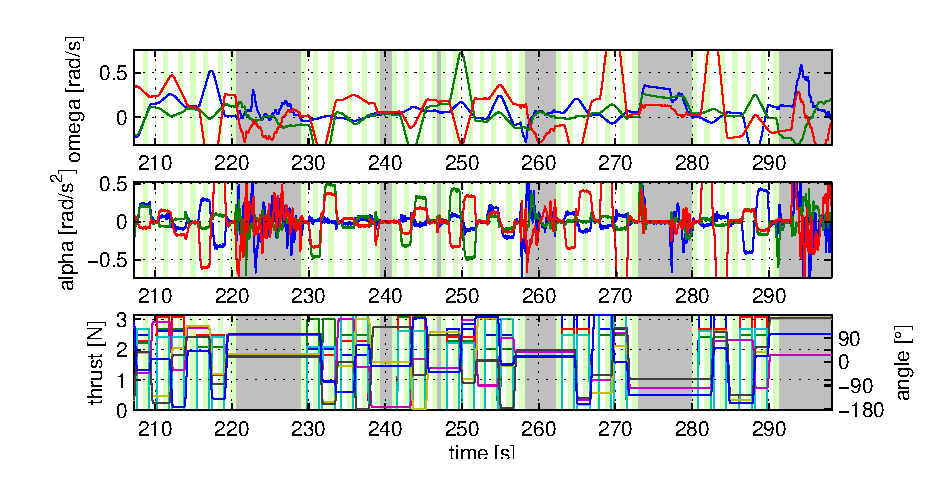
\includegraphics[scale=0.8]{images/interactive_cut/interactive_cut_long_modified.eps}
\caption{Except of dataset after transient marking}
\end{figure}
Then the segments where the blimp has been catched and repositioned need to be cut from the dataset. \\
For this purpose a semi-automatic cutting tool was implemented. 
The tool first identifies the segments of interest and then displays each of them to the use for visual inspection.
The user can then adjust the borders of the segments to cut away any undesired disturbances. \\
Good and bad segments are easily distinguished by looking at the angular acceleration plot.
An undisturbed system shows constant angular accelerations during the periods when the thrusters are active. \\
Using this approach to recording a dataset from Skye, only about 50\% of the raw data from the session has to be discarded.
The result is a dataset with undisturbed system response including transients.
When the described transient removal is applied about 40\% of transient-free data remains.\\
To summarize: for 10 seconds of transient-free data about 50 seconds of raw data has to be collected.

\begin{figure}[htbp]
\centering
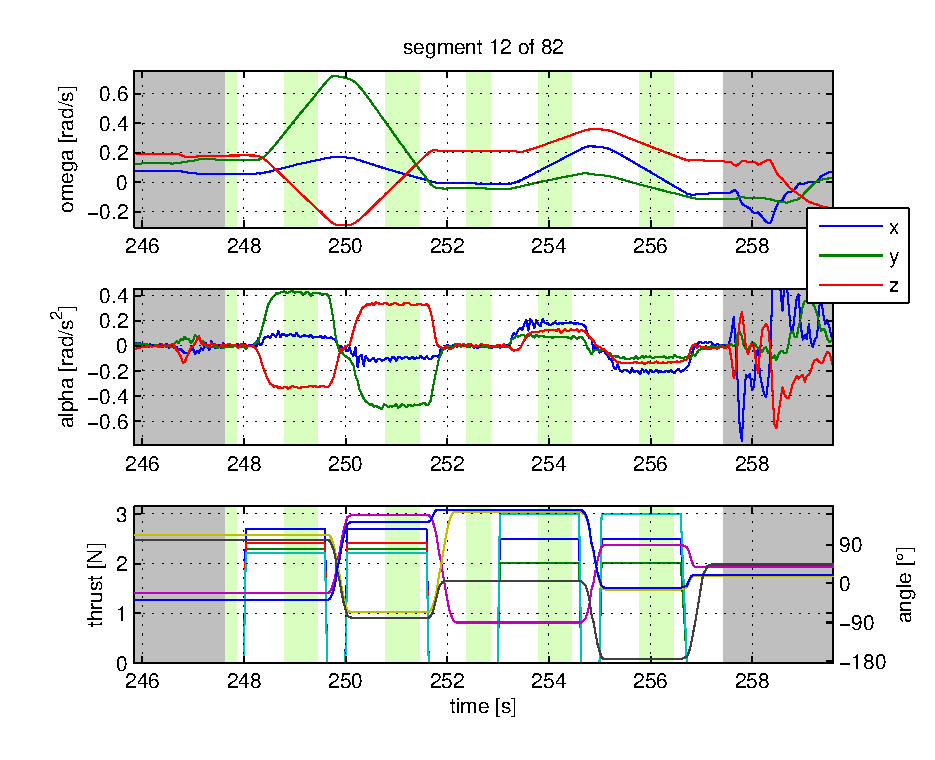
\includegraphics[scale=0.8]{images/interactive_cut/interactive_cut_detail_modified.eps}
\caption{Cutting tool displaying one segment of the dataset. 
\textbf{Grey} regions are discarded, \textbf{green} regions show steady-state response.
The legend of the thrust and angle plot has been removed for clarity. The important thing about this plot is that the traces with smooth transitions are the angles from the individual actuators and the other traces show the thrust force of each actuator.
Disturbances can be clearly seen in the greyed out areas.
The batch optimisation algorithm will use only the data from the green regions.}
\end{figure}

\section{Simulation}
\label{sec:simulation}
We also implemented a blimp simulator for several reasons:
\begin{itemize}
\item fast turn around time for generating new datasets
\item effects like noise and drag can be easily turned on and off
\item arbitrary blimp configurations can be created
\end{itemize}
We then came up with a list of requirements:
\begin{itemize}
\item include aerodynamic drag
\item include sensor noise
\item include thruster dynamics
\item allow for easy reconfiguration of the blimp
\end{itemize}
These requirements led us to the following implementation with object oriented \textsc{MATLAB} code:\\

The blimp is built with objects that interact with each other.
Each of these objects can have continuous and discrete states.\\
The simulator then interacts with the objects over a standardized interface.
At each time-step the simulator updates the states of the objects and then calls a function on each object to calculate the derivatives of the continuous states.
Additionally, at the border of a discrete time step the simulator also calls a function on the objects to get the next discrete states.\\

\begin{figure}[htbp]
\centering
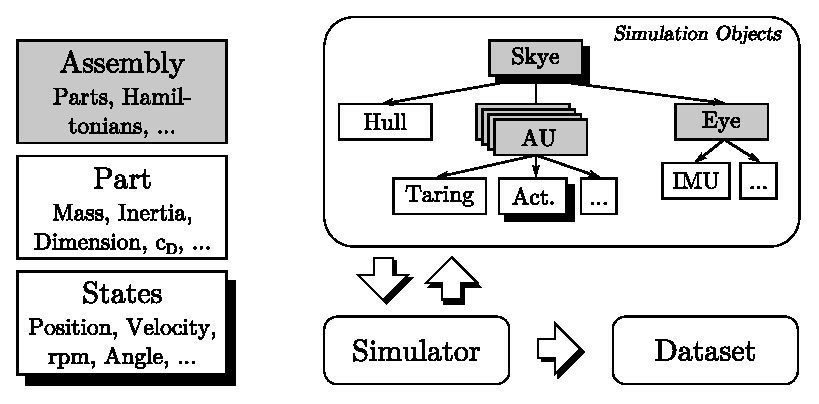
\includegraphics[width=0.9\textwidth]{images/sim/sim_tree.eps}
\caption{Tree like data-structure of simulation objects. Assembly parts (\textbf{gray}) have subparts (\textbf{white}) and hold additional information about their arrangement. Some parts includes states (\textbf{shaded}). The simulator interacts with the simulation objects and generates a dataset.}
\label{fig:sim_tree}
\end{figure}

\subsection{Motion Equation}
\label{sub:motion_equation}
At the core of the blimp simulation is a the rigid body dynamics model. \\
The simulator uses the same motion equation as described in table~\ref{tab:sys_mod}.\\

\subsection{Mechanical Properties}
\label{sub:mech_properties}
To calculate the mechanical properties, the blimp structure is represented in a tree like data-structure. (See figure~\ref{fig:sim_tree})\\
The root node of the tree is the actual rigid body object which is simulated by the simulator.\\
Each node in the tree represents an assembly of parts.
With this methodology the blimp is actually an assembly of several parts. 
In general it will include a hull, the electronics unit and a number of actuation units.
Each of these parts are assemblies by themselves.
The electronics unit could include for example the cover, a camera and the PX4 FMU, which simulates the sensors.\\
An actuation unit is also an assembly of for instance a battery, a taring weight and an actuator which simulates the actuator dynamics and generates the forces.\\
This concept allows to have different types of components in a library which can then be used to build an arbitrary blimp.\\
After the blimp has been assembled the mechanical properties of the parts at the leafs of the tree data-structure are recursively combined into their parent node.
This way the mechanical properties of the root node are recalculated.\\
The taring routine uses the tree structure to calculate values for the taring weights located at the actuation units. 
After taring is done, the changed mass of the taring weights cause the tree to recalculate the mechanical properties of the root node.

\subsection{Aerodynamic Drag}
\label{sub:aero_drag}
The aerodynamic effects are the most difficult part of modelling.
Aerodynamic drag is usually separated into \textit{form drag}, \textit{wall friction drag}, \textit{interference drag}, \textit{lift-induced drag} and \textit{wave drag} which are listed in decreasing importance for blimp modelling\footnote{
Wave drag describes compression effects of the fluid and is not relevant for subsonic speed.
Lift-induced drag is also neglected because blimps we consider blimps as symmetric profiles without considerable angle of attack.
Interference drag is assumed low, as the actuation units and other components on the blimp are much smaller than the hull and is therefore also neglected.
}.

We modelled form drag for translational movements and friction drag for rotational movements as quadratic functions w.r.t. to the velocity.
Further, a virtual mass factor was considered for the hull to consider the inertia of the surrounding fluid.
Form drag was applied to the hull and the actuation units which are represented by cylinders with appropriate dimension.
Friction drag was applied to the hull for rotational speed only.
Together with the form drag of the actuation units, the friction drag of the hull acts as a damping moment on rotational movements.
Form drag coefficients\footnote{
Blimps like Skye are close to the drag crisis point of spheres ($Re\approx3e05$). Interpolation according to the actual velocity is used.} and virtual mass factor were introduced according to the literature \citep{Kundu2012}.
The friction drag coefficient of the hull was determined such that the rotational aerodynamic resistance coincides with some reference measurements.
NOOOOOOOOOOO THIS HAS NOT BEEN DONE?
ALSO COMPARE WITH CHAPTER ABOVE.. XXXX

\subsection{Thruster Dynamics}
\label{sub:thrust_dynamics}
The actuator has been modelled according to test-bench measurements\footnote{Test-bench measurements have been done by Daniel Meier} of the thruster.
The dynamic thruster model includes:
\begin{itemize}
\item thrust start-up delay
\item thrust reaction delay
\item minimum and startup thrust thresholds
\item second order thrust motor dynamics
\item rotation actuator maximum speed
\item second order rotation actuator dynamics
\end{itemize}
Instead of trying to identify parameters with physical meanings (??ref to weichart??) a blackbox approach is used:
The minimal parameters needed to describe the listed properties of the thruster dynamics are matched to the test-bench measurements using an empirical approach.  \\
Because the thruster dynamics are not critical to our application this yields sufficient accuracy.

\subsection{Inertial Sensors Model}
\label{sub:imu_model}
Following the idea of the simulator framework the inertial sensors are also an object which is attached to the blimp assembly. \\
The framework of the mechanical structure goes both ways and motion of the rigid body at the root of the structure is distributed to each of the leaf nodes in their respective coordinate systems. \\
The sensor object then only has to take the already transformed accelerations, velocities and orientations and store them.
In this process the sensor object also adds noise to the sensor values.

